\chapter{Solving the wave equation with the FEM} \label{fem_waveq} 
\begin{flushright} {\tiny {\color{gray} chapter\_fem3.tex}} \end{flushright}
%~~~~~~~~~~~~~~~~~~~~~~~~~~~~~~~~~~~~~~~~~~~~~~~~~~~~~~~~~~~~~~~~~~~~~~~~~~~~~~~




%==============================================================================
\section{The wave equation}

Disclaimer: what follows in this section is greatly inspired 
by \url{https://en.wikipedia.org/wiki/Wave_equation} 

The wave equation is a second-order linear partial differential equation 
for the description of waves or standing wave fields such as mechanical waves 
(e.g. water waves, sound waves and seismic waves) or electromagnetic waves 
(including light waves). It arises in fields like acoustics, electromagnetism, and fluid dynamics. 

The wave equation is a hyperbolic partial differential equation,
and we will here focus on the scalar wave equation that 
represent the wave by a scalar $u(x,y,z,t)$.
The derivation of the wave equation is presented 
there\footnote{\url{https://en.wikipedia.org/wiki/Wave_equation}} 
and in virtually every physics textbook. The scalar wave equation is given by
\begin{equation}
\frac{\partial^2 u}{\partial t^2} = c^2 \left(
\frac{\partial^2 u}{\partial x^2} + 
\frac{\partial^2 u}{\partial y^2} + 
\frac{\partial^2 u}{\partial z^2} 
\right)
\label{eq:wavee1}
\end{equation}
where $c$ is a fixed non-negative real coefficient (the wave speed),
u is a scalar field representing a displacement from rest situation, e.g.
it could be gas pressure above or below normal, or the height of water in 
a pond above or below rest.

Note that sometimes you are likely to encounter different notations
for the 1st and 2nd-order derivatives:
\[
u_t = \partial_t u = \frac{\partial u}{\partial t} 
\qquad
u_{xx} = \frac{\partial^2 u}{\partial x^2} 
\]
so that Eq.~\eqref{eq:wavee1} then becomes
\[
u_{tt} = c^2(u_{xx}+u_{yy}+u_{zz})
\]

The equation states that at any given instance, at any given point, 
the acceleration of the displacement is proportional to the way the displacement's 
changes are squashed up in the surrounding area. In other words, a more pointy 
displacement gets pushed back more forcefully. 

This equation can also be written 
\begin{equation}
\frac{1}{c^2} \frac{\partial^2 u}{\partial t^2} = \Delta u
\end{equation}
or even 
\[
\Box u = 0 \qquad \text{with} \qquad \Box= \frac{1}{c^2} \frac{\partial^2 u}{\partial t^2} - \Delta
\]
in its most compact form, where $\Box$ is the d'Alembert 
operator\footnote{\url{https://en.wikipedia.org/wiki/D'Alembert_operator}}.


Solving the wave equation can be quite complicated. Still, it can be analyzed 
as a linear combination of simple solutions that are sinusoidal plane waves 
with various directions of propagation and wavelengths but all with the same propagation 
speed $c$. This analysis is possible because the wave equation is linear and homogeneous, 
so that any multiple of a solution is also a solution, and the sum of any two solutions 
is again a solution. This property is called the superposition principle in physics.


The wave equation alone does not specify a physical solution; 
a {\it unique} solution is usually obtained by setting a problem with further 
conditions, such as initial conditions, which prescribe the amplitude and phase of the wave. 
Another important class of problems occurs in enclosed spaces specified by boundary 
conditions, for which the solutions represent standing waves, or harmonics, analogous 
to the harmonics of musical instruments. 



%==============================================================================
\section{Solving the one-dimensional wave equation}

The one-dimensional wave equation simply writes
\[
\frac{\partial^2 u}{\partial t^2} = c^2 
\frac{\partial^2 u}{\partial x^2} 
\qquad \text{or}
\qquad 
u_{tt} = c^2 u_{xx}
\]
with $c>0$, to be solved on the domain $x \in [0,L_x]$.
The function u can be the displacement of a string or membrane of a drum, the height of a water wave or
air pressure for sound waves, dependent on the field the equation is used in.

The constant $c$ in the above equations defines the speed at which the wave ``moves''. 
To see this we can look at the one dimensional wave equation for which, if we have no 
other conditions, $u(x,t)=f(x+ct)$ and $u(x,t)=f(x-ct)$ are solutions if the function 
$f$ is twice differentiable. These two solutions have a constant shape which move in 
time with speed $c$ to the left and right respectively. A general solution to the one-
dimensional wave equation was actually derived by Jean le Rond d’Alembert \footnote{\url{https://en.wikipedia.org/wiki/Jean_le_Rond_d'Alembert}} (1717-1783) and is given 
by $u(x,t)=f(x-ct)+g(x+ct)$ being the sum of a left and right moving wave.




%-------------------------------------------
\subsection{Initial and boundary conditions}

Simply put, we need to specify the state of the system $u$ at the beginning, 
and since the domain in which the wave propagates is likely to be finite, 
also the boundary conditions.

For simplicity we will set
\begin{align}
u(x=0,t) & = 0 & \forall t\in \R^+  \nn\\
u(x=L_x,t) & = 0 & \forall t\in \R^+ \nn\\
u(x,0) &= u_0(x) & \forall x\in[0,L_x] \nn\\
u_t(x,0) &= u_1(x) & \forall x\in[0,L_x] \label{eq:fdm-wave-0}
\end{align}

Here, $u(x,t)$ represents the the displacement of a string (in one-dimension) or membrane of a drum (in
two-dimensions) that is held fixed at the boundary.


%-------------------------------------------
\subsection{A simple example: a standing wave \label{ss:sw1d}}

Let us set $L_x=1$ and $c=1$. Then one of the solutions is 
given by 
\[
x(x,t)=\cos(2\pi t) \sin(2\pi x)
\]
which is periodic in time with period 1 and is called a standing wave.
We also have
\[
u_t(x,t)=-2 \pi \sin (2\pi t) \sin(2\pi x)
\]
so that 
\begin{eqnarray}
u_0(x) &=& \sin(2\pi x) \\
u_1(x) &=& 0 
\end{eqnarray}
and the boundary conditions are respected: $u(0,t)=u(1,t)=0 \quad \forall t$.

\begin{center}
\includegraphics[width=4cm]{images/waveq/example1/u_0.pdf}
\includegraphics[width=4cm]{images/waveq/example1/u_1.pdf}
\includegraphics[width=4cm]{images/waveq/example1/u_2.pdf}
\includegraphics[width=4cm]{images/waveq/example1/u_3.pdf}\\
\includegraphics[width=4cm]{images/waveq/example1/u_4.pdf}
\includegraphics[width=4cm]{images/waveq/example1/u_5.pdf}
\includegraphics[width=4cm]{images/waveq/example1/u_6.pdf}
\includegraphics[width=4cm]{images/waveq/example1/u_7.pdf}\\
{\captionfont Solution at different times.}
\end{center}

%-----------------------------------------------------------------------------
\subsection{A few words about the FEM for the (1D) wave equation}

The finite element method is a numerical method generally used to solve differential equations with boundary
conditions. The concept of the finite element method is to divide the domain into finitely many smaller areas
called elements and approximate the solution of the differential equation on these elements using a suitable
set of basis functions. The result is a system of equations which can either be solved directly or by another
numerical method.


The finite element method has a few advantages over other numerical methods for solving differential equations (like the finite difference method). Firstly, the finite element method 
approximates the solution for
almost the whole domain, while most other methods only approximate the solution at a discrete set of
points. Secondly, with the finite element method we have more freedom over the discretization of the do-
main. We have the choice to increase precision at parts of the domain by using smaller elements and to
decrease the precision at parts by using larger elements. Thirdly we can choose different basis functions on
the elements to increase or decrease the precision at different parts of the domain or choose basis functions
which better approximate the actual solution, for example by using trigonometric functions instead of polynomials.

%-----------------------------------------------------------------------------
\subsection{Weak formulation}



First we will derive a different but equivalent formulation for the one-dimensional wave equation. 
Let $v(x)$ be a differentiable functions such that $v(0)=v(1)=0$ (i.e. zero on the boundaries
of the domain). By multiplying the wave equation with this function and integrating 
it over the domain we get following expression:
\[
\int_0^L  v(x) \left( \frac{\partial^2 u}{\partial t^2}(x,t) - c^2  
\frac{\partial^2 u}{\partial x^2}(x,t)\right) dx =0
\]

Let us recall the integration by parts formulation:
\[
\int_a^b u(x) v'(x) dx 
= [ u(x)v(x) ]_a^b  - \int_a^b u'(x) v(x) dx
= u(b)v(b)-u(a)v(a)  - \int_a^b u'(x) v(x) dx
\]
and use it on the equation above (only for the space derivative term):
\[
\int_0^L  v(x)  \frac{\partial^2 u}{\partial t^2}(x,t)  dx
- c^2 \int_0^L  v(x) \left(  \frac{\partial^2 u}{\partial x^2}(x,t)\right) dx =0
\]
\[
\int_0^L  v(x)  \frac{\partial^2 u}{\partial t^2}(x,t)  dx
- c^2 \left[ v(x)  \frac{\partial u}{\partial x}(x,t) \right]_0^ L
+c^2 \int_0^L  \frac{\partial v}{\partial x}(x,t)  \frac{\partial u}{\partial x}(x,t)  dx =0
\]
Since $v$ is zero on the boundary the middle term is then zero and we obtain:
\begin{equation}
\int_0^L  v(x)  \frac{\partial^2 u}{\partial t^2}(x,t)  dx
+c^2 \int_0^L  \frac{\partial v}{\partial x}(x,t)  \frac{\partial u}{\partial x}(x,t)  dx =0
\label{eq:fdm-wave-1}
\end{equation}
or, 
\[
a(u(x,t),v(x))=0
\]
with 
\begin{equation}
a(u(x,t),v(x)):=\int_0^L  v(x)  \frac{\partial^2 u}{\partial t^2}(x,t)  dx
+c^2 \int_0^L  \frac{\partial v}{\partial x}(x)  \frac{\partial u}{\partial x}(x,t)  dx
\label{eq:fdm-wave-aaa}
\end{equation}
For the integrals above to exist we require certain properties of $u,v$ and their derivatives.
For this we will use the $L_2$-norm on domain $D=[0,L]$. 
For a function $f$ this is defined by
\[
\| f \|_2 := \int_D  |f(x)|^2 dx 
\]
Using this norm a function $f$ is called square-integrable if the $L_2$-norm of $f$ 
is finite or more specifically:
\[
\|f\|_2 < \infty
\]
The set of all square-integrable functions is denoted by $L_2$. An important property of square-integrable
functions is that the integral of the product of two square-integrable functions over the domain D is also
finite. This property is important for the existence of the integrals above.

We want the functions $u,v$ and their first derivatives with respect to $x$ to be square-integrable. 
The set of functions which are square-integrable and whose first derivative is square-integrable 
is called a first order Sobolev space and can be denoted by $H^1$ . 
The set of functions which are also zero at the boundary of the domain is denoted by $H_0^1$.

We now want to find a function u which is in $H_0^1$ for each moment in time $t$ such that for every function $v$ in $H_0^1$ the equations of Eq.~\eqref{eq:fdm-wave-1} holds.
This gives rise to the weak formulation of our one-dimensional wave equation, which can now be stated as
follows

\vspace{.5cm}

\paragraph{Definition 1.1.1}
(Weak formulation). Find $u(x,t)$ such that for all $t\in \R$ it holds that $u(\cdot, t)\in H_0^1$ and for
all $v\in H_0^1$
\begin{equation}
a(u(x,t),v(x)) =0  \label{eq:fdm-wave-2}
\end{equation}
and the initial boundary conditions \eqref{eq:fdm-wave-0} holds.

\vspace{.5cm}

This is called the weak formulation since the function $u$ only has to verify Eq.~\eqref{eq:fdm-wave-2} with respect to certain functions $v$ called test functions.
Except for the derivation of the weak formulation above the rigorous connection between the weak formulation
and the ``strong formulation'' (i.e. the wave equation) is beyond the scope of this work.

%--------------------------------------------------
\subsection{Nodes and Elements}

We will now divide the interval $[0,L_x]$ into $nelx$ elements of equal size separated by $nnx=nelx+1$
nodes. 
The size of each element is given by $h=L_x/nelx$, so that the node coordinates can be defined as
\[
x_i := (i-1)h \qquad \text{for} \quad i=1,...nnx
\]
The nodes and elements are illustrated in the following figure:

\begin{center}
\begin{tikzpicture}
%\draw[fill=gray!23,gray!23](0,0) rectangle (11,2);
%\draw[step=0.5cm,gray,very thin] (0,0) grid (11,2); %background grid
\draw[thick] (0.5,1) -- (2,1)  ; 
\draw[thick,dashed] (2,1) -- (4,1)  ; 
\draw[thick] (4,1) -- (8,1)  ; 
\draw[thick,dashed] (8,1) -- (9.5,1)  ; 
\draw[thick,->] (9.5,1) -- (11,1)  ; 
\draw[] (1,0.8)--(1,1.2);
\draw[] (4,0.8)--(4,1.2);
\draw[] (5.5,0.8)--(5.5,1.2);
\draw[] (7,0.8)--(7,1.2);
\draw[] (10,0.8)--(10,1.2);
\node[] at (0.9,0.6) {\small $0$};
\node[] at (4,0.6) {\small $x_{i-1}$};
\node[] at (5.45,0.6) {\small $x_{i}$};
\node[] at (7,0.6) {\small $x_{i+1}$};
\node[] at (9.9,0.6) {\small $L_x$};
\node[] at (11,0.76) {\small $x$};
\draw[<->] (4,1.5)--(5.45,1.5);
\draw[<->] (5.55,1.5)--(7,1.5);
\node[] at (4.75,1.7) {\small $h$};
\node[] at (6.25,1.7) {\small $h$};
\end{tikzpicture}
\end{center}


%--------------------------------------------------
\subsection{Basis functions}


Instead of searching for a function $u$ in $H_0^1$ such that for all test functions 
$v$ in $H_0^1$ the equation of the weak formulation holds, 
we are going to search in a finite-dimensional subspace of $H^1$ . This space will consist
of those functions in $H^1$ which are piecewise polynomial on each element. 
We will restrict ourselves to piecewise linear functions for simplicity and 
we will denote this finite-dimensional set of functions as $S^1$.


The set $S^1$ will be defined as the functions $v$ that can be written as a linear 
combination of finitely many basis functions and that are zero at the boundaries. 
We will take $nnx$ basis functions, one for each node,
and call these $\bN_i(x)$ for $i=1, ..., nnx$. 
Then the functions $v$ in $S^1$ can be written as:
\begin{eqnarray}
v(x) &=& \sum_{i=1}^{nnx} \bN_i(x) \; v_i \qquad \text{with} \quad v_i \in \R, \quad v(0)=v(L_x)=0.
\end{eqnarray}

The basis functions can be written (for $i>1$ and $i<nnx$):
\begin{align}
\bN_i(x) &= 0 & \text{if } &x < x_{i-1} \nn\\
\bN_i(x) &=  \frac{x-x_{i-1}}{h}& \text{if } & x\in [x_{i-1},x_{i}] \nn\\
\bN_i(x) &=  \frac{x_{i+1}-x}{h}   & \text{if } &x \in [x_{i},x_{i+1}] \nn\\
\bN_i(x) &= 0 & \text{if } &x >x_{i+1} \nn
\end{align}
as shown in the following figure:
\begin{center}
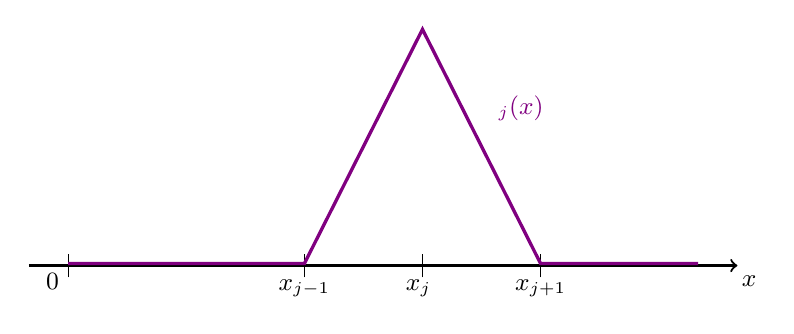
\begin{tikzpicture}
%\draw[fill=gray!23,gray!23](0,0) rectangle (11,4);
%\draw[step=0.5cm,gray,very thin] (0,0) grid (11,4); %background grid
\draw[thick,->] (0.5,1) -- (9.5,1)  ; 
\draw[-] (1,0.85) -- (1,1.15)  ; 
\draw[-] (4,0.85) -- (4,1.15)  ; 
\draw[-] (5.5,0.85) -- (5.5,1.15)  ; 
\draw[-] (7,0.85) -- (7,1.15)  ; 
\draw[very thick, violet] (1,1.025)--(4,1.025) -- (5.5,4) -- (7,1.025) --(9,1.025) ; 
\node[] at (6.75,3) {\small \color{violet} $\bN_j(x)$};
\node[] at (0.8,0.8) {\small $0$};
\node[] at (9.65,0.8) {\small $x$};
\node[] at (4,0.71) {\small $x_{j-1}$};
\node[] at (5.45,0.71) {\small $x_{j}$};
\node[] at (7,0.71) {\small $x_{j+1}$};
\end{tikzpicture}
\end{center}

Basis functions for $j=1$ and $j=nnx$ only contain the relevant half of the hat functions defined above.
Let us recall that an important property of these basis functions is that $\bN_i(x)$ is precisely one 
at node $x_i$ and zero on every other node.

%--------------------------------------------------------------------------
\subsection{Finite element solution}

Using the just defined basis functions we can define a finite element solution and finite element test functions as follows
\[
U(x,t) := \sum_{i=1}^{nnx} \bN_i(x)  U_i(t)
\]
\[
V(x) := \sum_{i=1}^{nnx} \bN_i(x)  V_i
\]

\paragraph{Definition 1.4.1} (Finite element formulation). 
Find $U(x,t)$ such that for all $t\in \R$ it holds that $U(\cdot,t)\in S^1$
and for all $V \in S^1$:
\[
a(U(x,t),V(x))=0
\]
and the following initial boundary conditions hold
\begin{align}
U(x=0,t) & = 0 & \forall t\in \R^+  \nn\\
U(x=L_x,t) & = 0 & \forall t\in \R^+ \nn\\
U(x,0) &= U_0(x) & \forall x\in[0,L_x] \nn\\
U_t(x,0) &= U_1(x) & \forall x\in[0,L_x] \label{eq:fdm-wave-4}
\end{align}
Note that because of the form $U$ takes, it does not have to hold that $U_0(x)$ equals $u_0(x)$.

For the finite element solution it is enough to test it only against the basis functions. This follows from the linearity of $a(u,v)$ in the second variable and therefore it holds that
\[
a(U(x,t),V(x))
=a\left(U(x,t), \sum_{i=1}^{nnx} \bN_j(x) V_j \right) 
=\sum_{i=j}^{nnx} V_j \; a\left(U(x,t),  \bN_j(x) \right) 
\]
Thus, if it holds for all of the basis functions $\bN_j$ , it also holds for all functions 
$V \in S^1$.

For each basis function $\bN_j(x)$ that is not on the edge, i.e. $j=2,...,nnx-1$ we can write using the definition of the bilinear form $a(\cdot,\cdot)$ (see Eq.~\eqref{eq:fdm-wave-aaa}):
\begin{eqnarray}
0 
&=& a\left(U(x,t),  \bN_j(x) \right)  \nn\\
&=&\int_0^L  \bN_j(x)  \frac{\partial^2 U}{\partial t^2}(x,t)  dx
+c^2 \int_0^L  \frac{\partial \bN_j}{\partial x}(x)  \frac{\partial U}{\partial x}(x,t)  dx \nn\\
&=&\int_0^L  \bN_j(x)  \frac{\partial^2 \left(\sum\limits_{i=1}^{nnx} \bN_i(x)  U_i(t) \right)}{\partial t^2}(x,t)  dx
+c^2 \int_0^L  \frac{\partial \bN_j}{\partial x}(x)  \frac{\partial \left(\sum\limits_{i=1}^{nnx} \bN_i(x)  U_i(t) \right)}{\partial x}(x,t)  dx \nn\\
&=&\sum\limits_{i=1}^{nnx} \frac{d^2  U_i(t) }{d t^2}  \int_0^L  \bN_j(x) \bN_i(x)   dx
+c^2 \sum\limits_{i=1}^{nnx} U_i(t)  \int_0^L  \frac{d \bN_j}{d x} (x) \frac{d \bN_i  }{d x}(x)  dx \nn\\
&=&\sum\limits_{i=1}^{nnx}   \ddot{U}_i(t)   \underbrace{\int_0^L  \bN_j(x) \bN_i(x)   dx}_{M_{ij}}
+c^2 \sum\limits_{i=1}^{nnx} U_i(t)  
\underbrace{\int_0^L  \frac{d \bN_j}{d x} (x) \frac{d \bN_i  }{d x}(x)  dx}_{K_{ij}} \nn\\
\end{eqnarray}
This results in $nnx-2$ linear ordinary differential equations.
For the two basis functions left out we can use
the boundary conditions imposed on $U$.
By defining the vector $\vec{\cal U}=(U_1(t),U_2(t),...U_{nnx}(t))$ 
we can use these $nnx$ linear differential equations to 
write the following ordinary differential equation
\begin{mdframed}[backgroundcolor=blue!5]
\begin{equation}
\M \cdot \vec{\ddot{{\cal U}}}(t) + c^2 \K \cdot \vec{\cal U}(t) = \vec{0}
\label{ss:waveq1}
\end{equation}
\end{mdframed}

The values of $M_{ij}$ and $K_{ij}$ can easily be calculated by splitting their integrals over all the elements like
\[
\int_0^{L_x} f(x) dx = \sum_{e=1}^{nelx} \int_{x_e}^{x_{e+1}} f(x) dx
\]
As the basis functions only have a maximum of two elements on which they are non-zero, the values of
Ti,j and Si,j can be calculated by just integrating over the few elements on which both basis functions are
non-zero. This allows us to calculate the following coefficients
\begin{eqnarray}
M_{i,i}&=&\int_0^L \bN_i(x) \bN_i(x) dx =\int_{x_{i-1}}^{x_{i+1}} \bN_i(x) \bN_i(x) dx = \frac23 h \nn\\
M_{i,i-1}&=&\int_0^L \bN_i(x) \bN_{i-1}(x)dx=\int_{x_{i-1}}^{x_{i}}\bN_i(x) \bN_{i-1}(x) dx=\frac16 h \nn\\
K_{i,i}&=&\int_0^L \bN_i'(x)\bN_i'(x) dx =\int_{x_{i-1}}^{x_{i+1}} \bN_i'(x) \bN_i'(x) dx = \frac{2}{h}\nn\\
K_{i,i-1}&=&\int_0^L \bN_i'(x)\bN_{i-1}'(x) dx =\int_{x_{i-1}}^{x_{i}} \bN_i'(x) \bN_{i-1}'(x) dx =-\frac{1}{h}
\end{eqnarray}
These integrals can easily be computed by hand in the 1D case but we will see that in most 2D,3D cases
this is not the case and we must resort to numerical quadrature.

%-----------------------------------------------------------------
\subsection{Time discretisation}

We can use a second-order approximation for the second-order derivative:
\[
\vec{\ddot{{\cal U}}}(t) \simeq  \frac{ \vec{\cal U}(t+ \delta t) -2 \vec{\cal U}(t) + \vec{\cal U}(t-\delta t)}{\delta t^2}
\]
which we can substitute in Eq.~\eqref{ss:waveq1}:
\[
\M \cdot \frac{ \vec{\cal U}(t+\delta t) -2 \vec{\cal U}(t) + \vec{\cal U}(t-\delta t)}{\delta t^2} 
+c^2 \K \cdot \vec{\cal U}(t) = \vec{0}
\]
Note that in the equation above the vector $\vec{\cal U}$ multiplying $\K$ is evaluated at time $t$. We will come back 
to this very shortly.
\[
\M \cdot ( \vec{\cal U}(t+\delta t) -2 \vec{\cal U}(t) + \vec{\cal U}(t- \delta t)) 
=- c^2 \delta t^2 \K \cdot \vec{\cal U}(t) 
\]
leading to finally write ({\color{orange} method \# 1}):
\begin{mdframed}[backgroundcolor=blue!5]
\[
\M \cdot  \vec{\cal U}(t+\delta t)
=\underbrace{ [2  \M  - c^2 \delta t^2 \K  ]  \cdot \vec{\cal U}(t) - \M \cdot \vec{\cal U}(t-\delta t)}_{\vec{b}}
\]
\end{mdframed}
which is of the form 
\[
{\cal \bm A} \cdot \vec{\cal U} (t+\delta t) = \vec{b}
\]
Alternatively we would have used an implicit approach by writing
\[
\M \cdot \frac{ \vec{\cal U}(t+\delta t) -2 \vec{\cal U}(t) + \vec{\cal U}(t-\delta t)}{\delta t^2} 
+c^2 \K \cdot \vec{\cal U}(t {\color{violet} +\delta t} ) = \vec{0},
\]
leading to write:
\begin{mdframed}[backgroundcolor=blue!5]
\[
(\M + c^2 \delta t^2 \K ) \cdot \vec{\cal U}(t+\delta t) = \underbrace{ \M \cdot(2 \vec{\cal U}(t) - \vec{\cal U}(t-\delta t)) }_{\vec{b}}
\] 
\end{mdframed}

\vspace{.5cm}

Given the presence of the terms $\vec{\cal U}(t)$ and $\vec{\cal U}(t-\delta t)$ in the equations above,
we can only solve the equation for $t \ge 2\delta t$ (assuming the time step $\delta t$ remains constant):
\[
\M \cdot  \vec{\cal U}(2\delta t)
= [2  \M  - c^2 \delta t^2 \K  ]  \cdot \vec{\cal U}(\delta t) - \M \cdot \vec{\cal U}(0)
\]
The value of $\vec{\cal U}(0)$ is known as it is the field at $t=0$ (initial condition). 
However, quid of $\vec{\cal U}(\delta t)$?
One way to avoid this problem is by using a 1st order Taylor expansion of this term:
\[
\vec{\cal U}(\delta t) = \vec{\cal U}(0) + \delta t \; \vec{\dot{{\cal U}}}(0)
\]
and since we know both terms in the rhs then all is well.

\vspace{.6cm}

Another approach can be taken ({\color{orange} method \# 2}): let us define 
\[
\vec{\cal V}=
\frac{ \vec{\cal U}(t+\delta t) -2 \vec{\cal U}(t) + \vec{\cal U}(t-\delta t)}{\delta t^2} 
\]
Then one needs to solve two equations one after the other:

\begin{mdframed}[backgroundcolor=blue!5]
\begin{eqnarray}
\M \cdot \vec{\cal V} &=&  -c^2 \K \cdot \vec{\cal U}(t) \nn\\
\vec{\cal U}(t+\delta t) &=& \delta t^2 \; \vec{\cal V} +2 \vec{\cal U}(t) - \vec{\cal U}(t-\delta t)
\end{eqnarray}
\end{mdframed}


\vspace{.6cm}

There is yet another option ({\color{orange} method \# 3}). 
Let us define this time $\vec{\cal W}(t)=\vec{\dot{{\cal U}}}(t)$.
Then Eq.~\eqref{ss:waveq1} can be written 
\[
\vec{\dot{{\cal W}}}(t) = \vec{\ddot{{\cal U}}} = -c^2 \M^{-1} 
\cdot \K \cdot \vec{\cal U}(t)
\]
Then we must solve the coupled set of equations:
\begin{align}
\vec{\dot{{\cal U}}}(t) &= \vec{\cal W}(t) \\
\vec{\dot{{\cal W}}}(t) &= -c^2 \M^{-1} \cdot \K \cdot \vec{\cal U}(t) 
\end{align}
with initial values
\begin{align}
\vec{\cal U}(0) &= \vec{\cal U}_0 \\ 
\vec{\cal W}(0) &= \vec{\dot{{\cal U}}}_0
\end{align}
We can also write (to first order)
\begin{align}
\frac{\vec{\cal U}(t+dt)-\vec{\cal U}(t) }{dt}    &= \vec{\cal W}(t) \\
\M \cdot \frac{\vec{\cal W}(t+dt)-\vec{\cal W}(t) }{dt}  &= -c^2 \; \K \cdot \vec{\cal U}(t) 
\end{align}
and finally
\begin{mdframed}[backgroundcolor=blue!5]
\begin{align}
\vec{\cal U}(t+dt) = \vec{\cal U}(t) + dt \; \vec{\dot{{\cal U}}}(t) \\
\M \cdot \frac{\vec{\dot{{\cal U}}}(t+dt)-\vec{\dot{{\cal U}}}(t) }{dt}  &= -c^2 \K \cdot \vec{\cal U}(t) 
\end{align}
\end{mdframed}
The first equation is straightforward and we then solve the second equation in a similar 
was as in method 2 to obtain $\vec{\dot{{\cal U}}}(t+dt)$.

Concretely, it goes as follows. Let us define 
$\vec{\cal R}= (\vec{\dot{{\cal U}}}(t+dt)-\vec{\dot{{\cal U}}}(t) )/dt$.
Then the second equation is $\M \cdot \vec{\cal R} = -c^2 \; \K \cdot \vec{\cal U}(t)$ 
and the algorithm goes 
as follows:
\begin{enumerate}
\item $\vec{\cal U}(t+dt) = \vec{\cal U}(t) + dt \; \vec{\dot{{\cal U}}}(t)$
\item solve $\M \cdot \vec{\cal R} = -c^2 \; \K \cdot \vec{\cal U}(t)$ 
\item recover $\vec{\dot{{\cal U}}}(t+dt) = \vec{\dot{{\cal U}}}(t) + dt \; \vec{\cal R}$
\end{enumerate}
This method is different than the other two because it keeps $\vec{\cal U}$ 
and its time-derivative as unknowns. 

Note that in all three cases the FE matrix is simply the mass matrix, 
which is good news since it tends to be nicely conditioned and symmetric.

This is all implemented in \stone~164. 

%-----------------------------------------------------
\subsection{The case of non-equidistant nodes and/or higher order elements}

In this section we will generalize the finite element method by first allowing irregular elements, i.e. 
elements of different size:
\begin{center}
\begin{tikzpicture}
%\draw[fill=gray!23,gray!23](0,0) rectangle (11,2);
%\draw[step=0.5cm,gray,very thin] (0,0) grid (11,2); %background grid
\draw[thick] (0.5,1) -- (2,1)  ; 
\draw[thick,dashed] (2,1) -- (4,1)  ; 
\draw[thick] (4,1) -- (8,1)  ; 
\draw[thick,dashed] (8,1) -- (9.5,1)  ; 
\draw[thick,->] (9.5,1) -- (11,1)  ; 
\draw[] (1,0.8)--(1,1.2);
\draw[] (4,0.8)--(4,1.2);
\draw[] (5.5,0.8)--(5.5,1.2);
\draw[] (7.5,0.8)--(7.5,1.2);
\draw[] (10,0.8)--(10,1.2);
\node[] at (0.9,0.6) {\small $a$};
\node[] at (4,0.6) {\small $x_{i-1}$};
\node[] at (5.45,0.6) {\small $x_{i}$};
\node[] at (7.5,0.6) {\small $x_{i+1}$};
\node[] at (9.9,0.6) {\small $b$};
\node[] at (11,0.76) {\small $x$};
\draw[<->] (4,1.5)--(5.45,1.5);
\draw[<->] (5.55,1.5)--(7.5,1.5);
\node[] at (4.75,1.7) {\small $h_{i-1}$};
\node[] at (6.5,1.7) {\small $h_i$};
\end{tikzpicture}
\end{center}

We divide an interval [a,b] with $a<b$ into $nelx$ elements separated by nodes. 
The nodes $x_i$ with $i=1,...nnx$ are chosen such that $a=x_1<x_2<...<x_{nnx-1} < x_{nnx}=b$
and the elements can then defined as
\[
e_i = [x_i,x_{i+1}] \qquad \text{for} \quad i=1,...,nnx
\]
with its size $h_i:=x_{i+1}-x_i$.

We have now two choices: either we define a so-called reference element (sometimes also called
canonical element) and establish the mapping from any real element to the reference one, later to be used in the 
formulation of the integrals, or we express the basis functions locally for each element and proceed by using these 
in the integrals.

For example the basis functions would then write 
\begin{align}
\bN_i(x) &= 0 & \text{if } &x < x_{i-1} \nn\\
\bN_i(x) &=  \frac{x-x_{i-1}}{x_i-x_{i-1}}& \text{if } & x\in [x_{i-1},x_{i}] \nn\\
\bN_i(x) &=  \frac{x_{i+1}-x}{x_{i+1}-x_i}   & \text{if } &x \in [x_{i},x_{i+1}] \nn\\
\bN_i(x) &= 0 & \text{if } &x >x_{i+1} \nn
\end{align}
as shown in the following figure:
\begin{center}
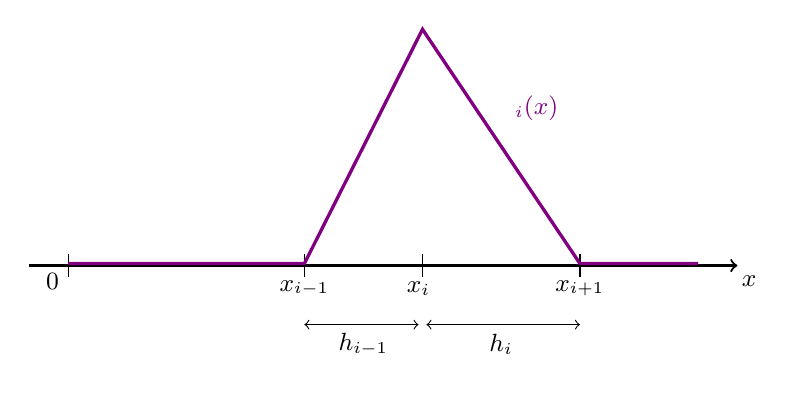
\begin{tikzpicture}
%\draw[fill=gray!23,gray!23](0,0) rectangle (11,4);
%\draw[step=0.5cm,gray,very thin] (0,0) grid (11,4); %background grid
\draw[thick,->] (0.5,1) -- (9.5,1)  ; 
\draw[-] (1,0.85) -- (1,1.15)  ; 
\draw[-] (4,0.85) -- (4,1.15)  ; 
\draw[-] (5.5,0.85) -- (5.5,1.15)  ; 
\draw[-] (7.5,0.85) -- (7.5,1.15)  ; 
\draw[very thick, violet] (1,1.025)--(4,1.025) -- (5.5,4) -- (7.5,1.025) --(9,1.025) ; 
\node[] at (6.95,3) {\small \color{violet} $\bN_i(x)$};
\node[] at (0.8,0.8) {\small $0$};
\node[] at (9.65,0.8) {\small $x$};
\node[] at (4,0.71) {\small $x_{i-1}$};
\node[] at (5.45,0.71) {\small $x_{i}$};
\node[] at (7.5,0.71) {\small $x_{i+1}$};

\draw[<->] (4,0.25)--(5.45,0.25);
\draw[<->] (5.55,0.25)--(7.5,0.25);
\node[] at (4.75,0) {\small $h_{i-1}$};
\node[] at (6.5,0) {\small $h_i$};
\end{tikzpicture}
\end{center}

Otherwise we would normally define the reference element $r=[-1,+1]$ and the 
basis functions inside the element attached to each node would be given by
\begin{eqnarray}
\bN_1(r) &=& \frac12 (1-r) \\
\bN_2(r) &=& \frac12 (1+r) 
\end{eqnarray}
We have of course already encountered these in Section~\ref{XYZ}.


The topic of higher-order elements has been covered in Section~\ref{} and poses no 
real difficulty. For example, 2nd-order elements would require an additional 
node in the middle of each element while the basis functions are defined on 
the reference element in section REF ... 

%-------------------------------------------------------------------------------------
\subsection{Conservation of energy}


The concept of conservation of energy is used all over physics and states most of the time that the total
amount of energy in a closed systems is constant. This conservation can also hold for the one-dimensional
wave equation and can be formulated as

\paragraph{Theorem} For a solution $u$ of the one-dimensional
wave equation there exists a constant $C>0$, independent of time $t$, such that
\begin{equation}
\left\|  \frac{\partial u}{\partial t} (\cdot, t)  \right\|^2 + 
c^2 \left\|  \frac{\partial u}{\partial x} (\cdot, t)  \right\|^2 =C \label{eq:fdm-wave-5}
\end{equation}
where $\| \cdot \|$ is the $L_2$-norm over the domain. 

\vspace{.5cm}

Proof: Let $v(x,t)=\frac{\partial u}{\partial t}(x,t)$ be the test function in the weak formulation of the one-dimensional wave equation. Using Eq.~\eqref{eq:fdm-wave-aaa}, this gives
\begin{eqnarray}
0 
&=& \int_D v(x,t) \frac{\partial^2 u}{\partial t^2}(x,t) dx + c^2 \int_D  \frac{\partial u}{\partial x}  \frac{\partial v}{\partial x} dx \nn\\
&=& \int_D \frac{\partial u}{\partial t}(x,t) \frac{\partial^2 u}{\partial t^2}(x,t) dx + c^2 \int_D  \frac{\partial u}{\partial x}  \frac{\partial }{\partial x} \frac{\partial u}{\partial t}(x,t) dx \nn\\
&=& \int_D \frac12 \frac{\partial}{\partial t} \left(\frac{\partial u}{\partial t} \right)^2 dx + c^2
\int_D  \frac12 \frac{\partial}{\partial t} \left( \frac{\partial u}{\partial x}  \right)^2  dx \nn\\
&=& \frac12 \frac{\partial}{\partial t} \int_D  \left(\frac{\partial u}{\partial t} \right)^2 dx + c^2
\frac12 \frac{\partial}{\partial t} \int_D   \left( \frac{\partial u}{\partial x}  \right)^2  dx \nn\\
&=& \frac12 \frac{\partial}{\partial t} 
\left(
\left\|  \frac{\partial u}{\partial t} (\cdot, t)  \right\|^2 + 
c^2 \left\|  \frac{\partial u}{\partial x} (\cdot, t)  \right\|^2
\right)
\end{eqnarray}
which implies Eq.~\eqref{eq:fdm-wave-5}.
This implies conservation of energy for the finite element solution of the wave equation.

From the above formulas we can define an energy function as $E(u,t)=\|\dot{u}\|^2  + c^2 \| \partial_x u \|^2 $, such that for a solution $u$ of the weak or finite element formulation there exists a constant $C>0$ 
such that $E(u,t)=C$ for all $t$.

Considering now the discrete solution $U$, the first error we can notice is that the initial values of the wave equation $u(x,0)$ and $\partial_t u(x,0)$ and its discretized value for the finite element formulation 
$U(x,0)$ and $\partial_t U(x,0)$ do not necessarily have the same energy,
or more specific, $E(u,0)$ and $E(U,0)$ do not have to be equal. But if we make the elements smaller and use
higher order polynomials for approximation, we can better approximate the original initial value with $U$ and
$\partial_t U$ and therefore better approximate the energy.

To analyse what happens to the energy when we discretize in time the system of ordinary differential equations
of Eq.~\eqref{ss:waveq1} we can use a more efficient way of calculating the energy. We can get this by putting the finite element $U(x,t)=\sum_{i=1}^{nnx} \bN_i(x) U_i(t)$ in the energy function, resulting in the following equations:

\begin{eqnarray}
E(U,t) 
&=& \left\|  \frac{\partial u}{\partial t} (\cdot, t)  \right\|^2 + 
c^2 \left\|  \frac{\partial u}{\partial x} (\cdot, t)  \right\|^2 \nn\\
&=& \int_D \left( \sum_{i=1}^{nnx} \bN_i(x) \dot{U}_i(t) \right)^2 dx 
+ c^2 \int_D \left( \sum_{i=1}^{nnx} \frac{d \bN_i}{dx}(x) U_i(t) \right)^2 dx \nn\\
&=& \int_D \sum_{i=1}^{nnx}\sum_{j=1}^{nnx} \bN_i(x) \bN_j(x) \dot{U}_i(t) \dot{U}_j(t) dx
+ c^2 \int_D \sum_{i=1}^{nnx}\sum_{j=1}^{nnx} \frac{d \bN_i}{dx}(x) \frac{d \bN_j}{dx}(x) U_i(t) U_j(t) dx\nn\\
&=& \sum_{i=1}^{nnx}\sum_{j=1}^{nnx} \dot{U}_i(t) \dot{U}_j(t)  \int_D  \bN_i(x) \bN_j(x) dx
+ c^2 \sum_{i=1}^{nnx}\sum_{j=1}^{nnx} U_i(t) U_j(t) \int_D  \frac{d \bN_i}{dx}(x) \frac{d \bN_j}{dx}(x)  dx\nn\\
&=& \sum_{i=1}^{nnx}\sum_{j=1}^{nnx} \dot{U}_i(t) \dot{U}_j(t) M_{ij} 
+ c^2 \sum_{i=1}^{nnx}\sum_{j=1}^{nnx} U_i(t) U_j(t) K_{ij} dx \nn\\
&=& \vec{\dot{{\cal U}}}^T \cdot \M \cdot \vec{\dot{{\cal U}}} 
+ c^2 \; \vec{\cal U}^T \cdot \K \cdot \vec{\cal U}
\end{eqnarray}
We see that methods 1\&2 might not be convenient when it comes to energy calculations since 
the time derivative of the $\vec{\cal U}$ vector does not appear explicitly, while it does
in method 3.

Because we know that real solutions of the wave equation and finite element formulation need to have a
constant energy, we can use the energy function as a measure of error over time when we have all the values
$U_i$ and $\dot{U}_i$ at a moment in time, like for the third method. We can even use this method this analyse
numerical solutions for which we don’t have the analytical solutions.

%---------------------------------------------------
\subsection{time step value \& CFL condition}






:




\newpage
%==============================================================================
\section{Solving the two-dimensional wave equation}




It simply writes
\[
\frac{\partial^2 u}{\partial t^2} = c^2 
\left( 
\frac{\partial^2 u}{\partial x^2} + 
\frac{\partial^2 u}{\partial y^2} 
\right)
\]
or also sometimes
\[
u_{tt} = c^2 (u_{xx} + u_{yy})
\]
Here to initial conditions and boundary conditions must be provided.


{\color{red} ... include here weak form derivation and discretisation ... }

We arrive again at the following equation
\begin{equation}
\M \cdot \vec{\ddot{{\cal U}}}(t) + c^2 \K \cdot \vec{\cal U}(t) = \vec{0}
\label{ss:waveq2d}
\end{equation}
At this stage a decision must be made, i.e. whether quadrilaterals or triangles 
are used, and whether they are linear, quadratic, etc ...



